\documentclass[12pt]{beamer}
\usetheme{Hannover}
\usepackage{graphicx}
\usepackage{booktabs}
\usepackage[english]{babel}
\usepackage{kotex}
%\usepackage[pdfencoding=auto]{hyperref}
\hypersetup{pdfencoding=auto}
\usepackage{ulem}
\usepackage[per-mode=symbol]{siunitx}
\sisetup{inter-unit-product =$\cdot$}
\usepackage{color}
\usepackage{ulem}
\usepackage{amsmath,amssymb}
\graphicspath{{images/}}
\title[\LaTeX - Contribution]{\LaTeX 입문 - Contribution}

\author{경기과학고 \TeX 사용자협회}
\institute[GSHSTeXSociety]{\url{latex.gs.hs.kr}}
\date{마지막 수정일 : \today}

\setbeamertemplate{navigation symbols}{}%to suppress navigation tools

%\AtBeginSection[]{
%	\begin{frame}
%		\vfill
%		\centering
%		\begin{beamercolorbox}[sep=8pt,center,shadow=true,rounded=true]{title}
%			\usebeamerfont{title}\insertsectionhead\par%
%		\end{beamercolorbox}
%		\vfill
%	\end{frame}
%}

\begin{document}

\begin{frame}
\titlepage % Print the title page as the first slide
\end{frame}
\section{개요}
\begin{frame}{본 문서의 목적}
	본 문서는 경기과학고 구성원들의 협회 활동 참여 장려에 목적이 있다.
	협회 활동에 참여하고자 하는 구성원들은 이 문서를 통해
	\begin{itemize}
		\item 협회 활동 참여 시 염두에 두어야 할 것들
		\item 협회 활동 참여에 필요한 것들
	\end{itemize}
	을 알아갈 수 있다.
	\vfill
	이 문서는 협회 규범집(\url{https://git.io/vMb68})을 기반으로 제작되었다.
	\vfill
\end{frame}
\section{협회}
\subsection{협회의 목적}
\begin{frame}{협회의 목적}
	협회가 있기 전에는\ldots
	\begin{itemize}
		\item \TeX 의 높은 진입장벽, learning curve
		\item R\&E 보고서 \TeX 양식의 오류
		\begin{itemize}
			\item 초보자는 오류를 직접 고치기 어려움
			\item 오류를 고친다 하더라도, 공지/배포가 어려움
		\end{itemize}
	\end{itemize}
\end{frame}
\begin{frame}{협회의 목적}
	협회를 통하여\ldots
	\begin{itemize}
		\item 초심자와 숙련자의 win-win
		\begin{itemize}
			\item 초심자 : 입문서, 워크샵을 통해 쉽게 배움
			\item 숙련자 : 입문서 제작을 통한 정리, 추가학습
		\end{itemize}
		\item 오픈소스
		\begin{itemize}
			\item 학생/교사 모두에게 열려있는 편집 권한
			\item 참여하는 저자에게도 큰 도움이 됨
		\end{itemize}
		\item 중앙집권화
		\begin{itemize}
			\item 빠른 오류 제보 및 처리
			\item 홈페이지를 통한 안내
			\item 텍 사용자간 교류(사용 팁 공유)
		\end{itemize}
	\end{itemize}
\end{frame}
\subsection{협회의 구조}
\begin{frame}{협회의 구조}
	\begin{figure}[h]
		\centering
		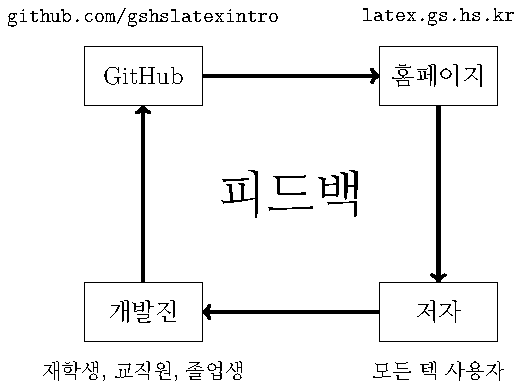
\includegraphics[width=\textwidth]{gshstexsociety_structure.pdf}
	\end{figure}
\end{frame}
\subsection{GitHub}
\begin{frame}{GitHub}
	\begin{itemize}
		\item GitHub[깃허브], \url{github.com}
		\item 단순한 코드 공유 사이트가 아님.
		\item git을 통한 코드 버전관리 및 협업 코딩
	\end{itemize}
	\begin{center}
		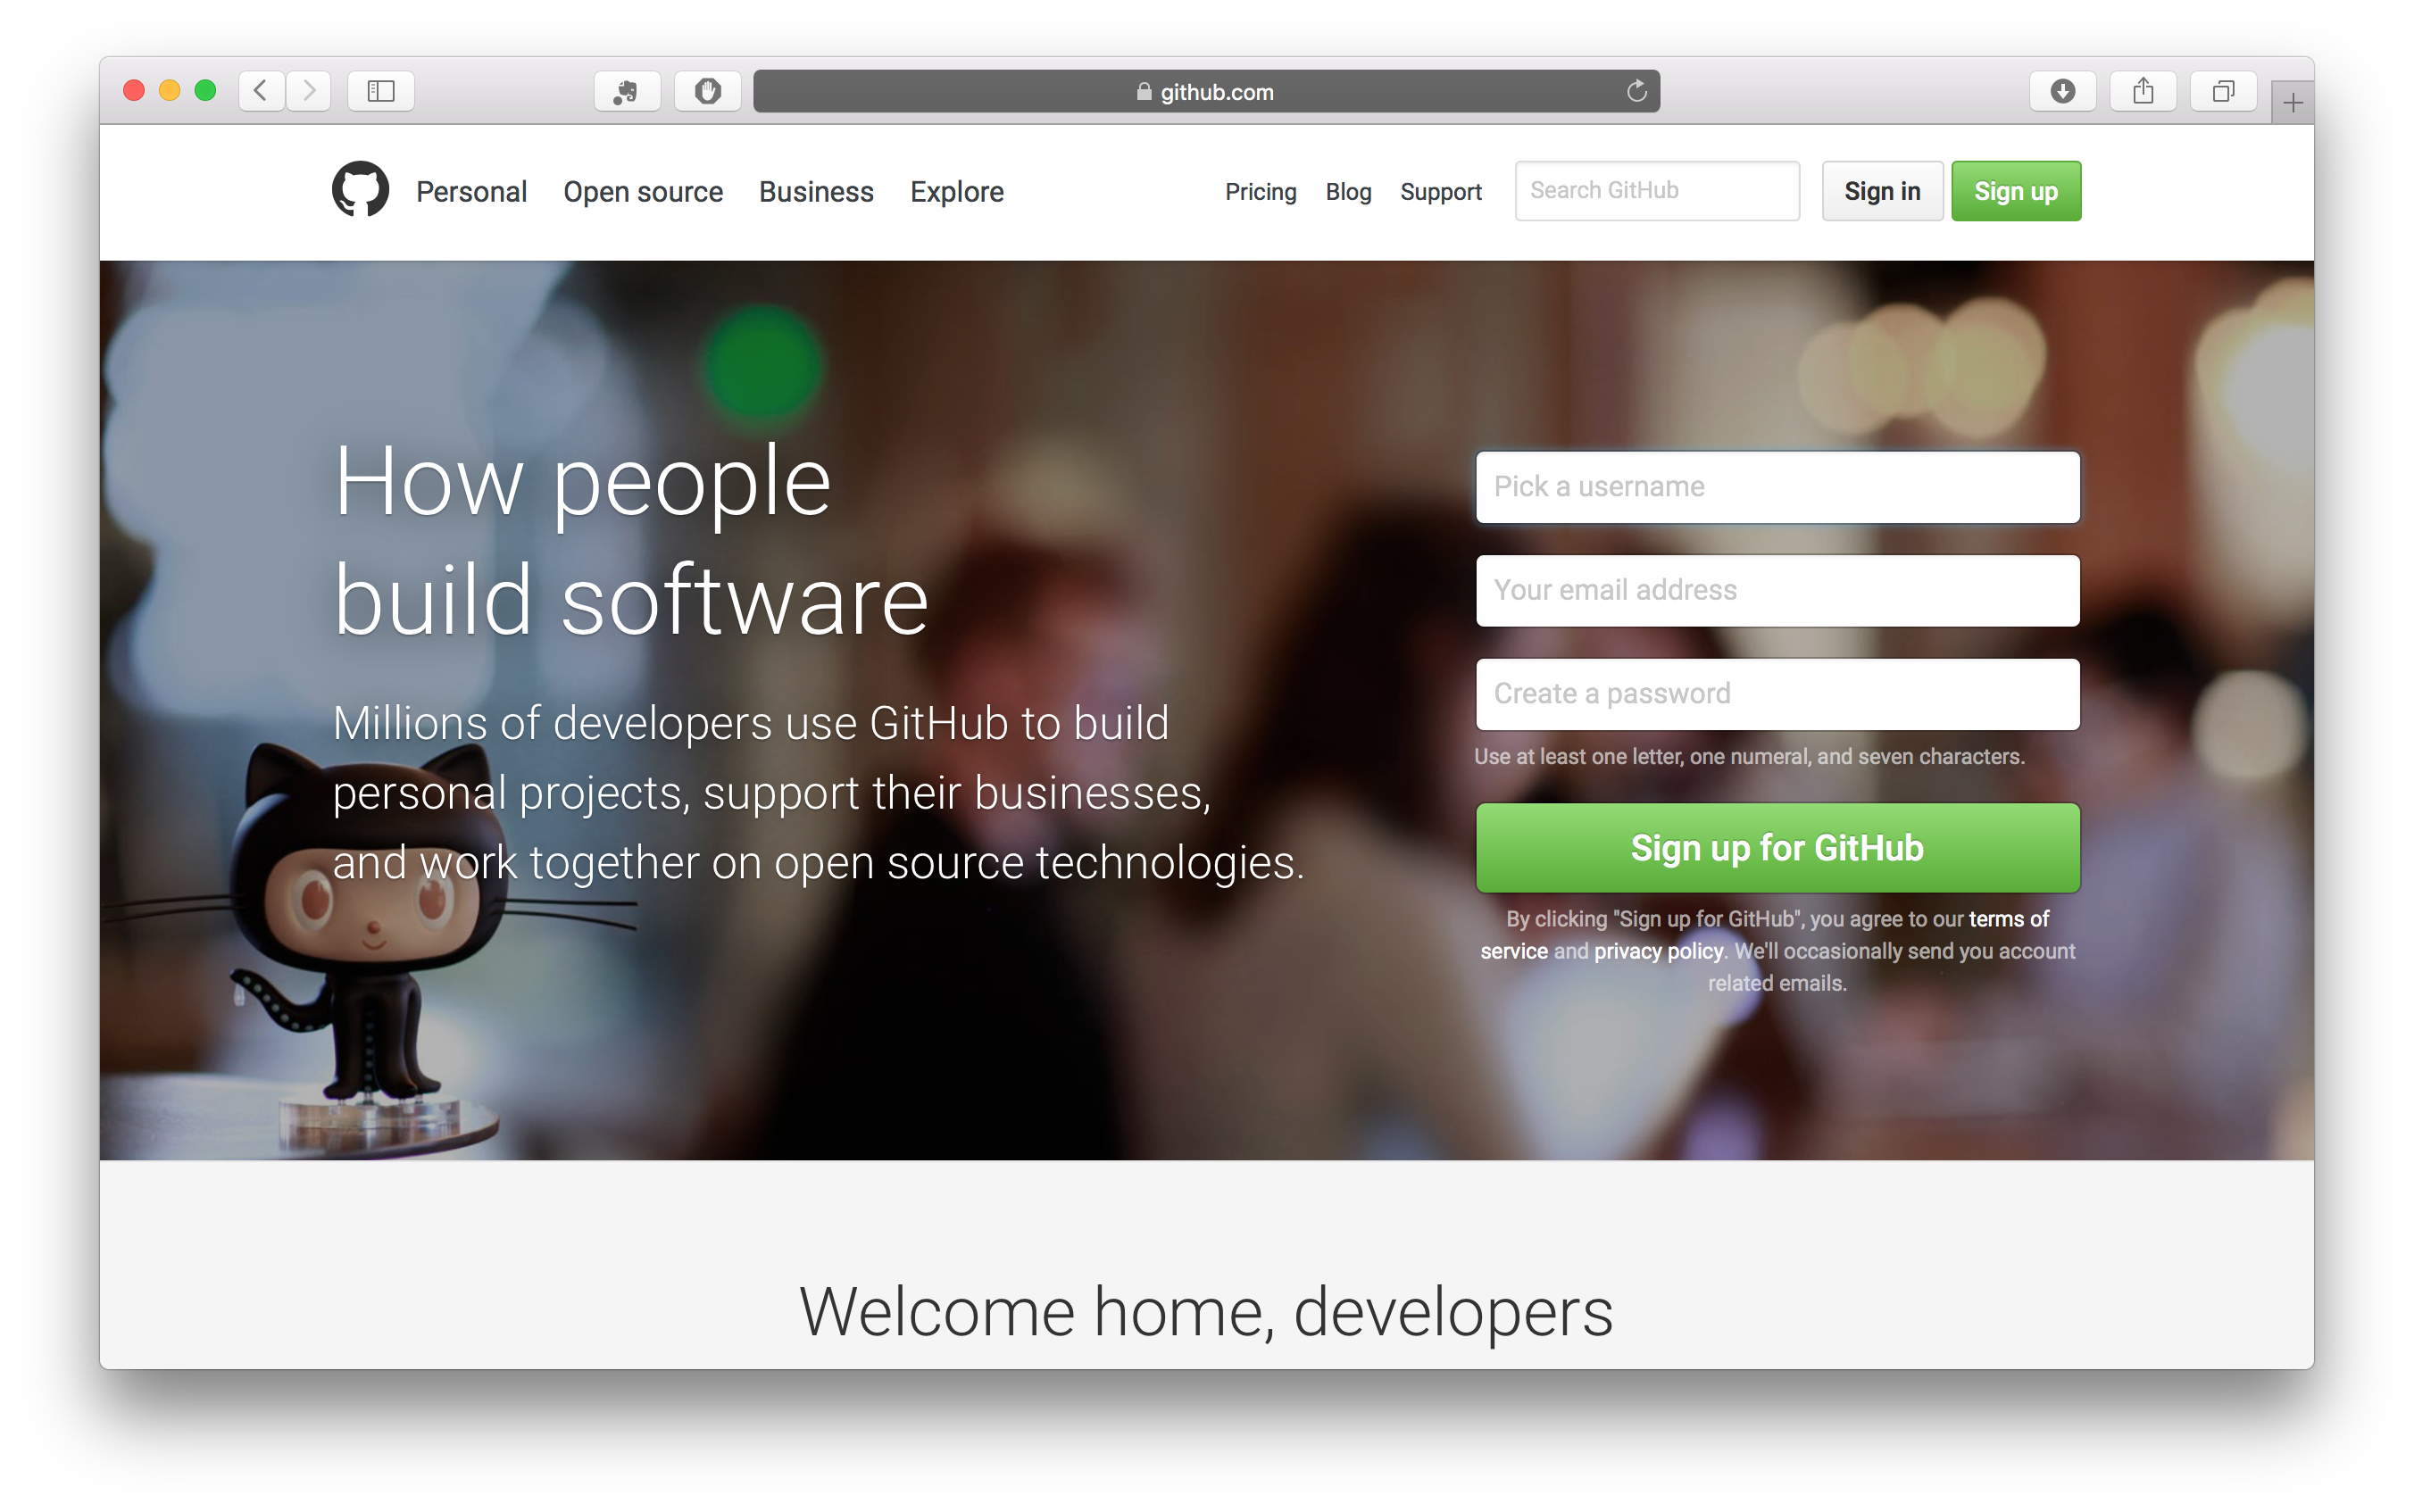
\includegraphics[width=\textwidth]{GitHub_website.png}
	\end{center}
\end{frame}
\begin{frame}{GitHub}
	\framesubtitle{GitHub를 통한 협업}
	\begin{itemize}
		\item 영어 사이트이지만 큰 어려움은 없음
		\item \url{github.com/gshslatexintro}
	\end{itemize}
	\begin{center}
		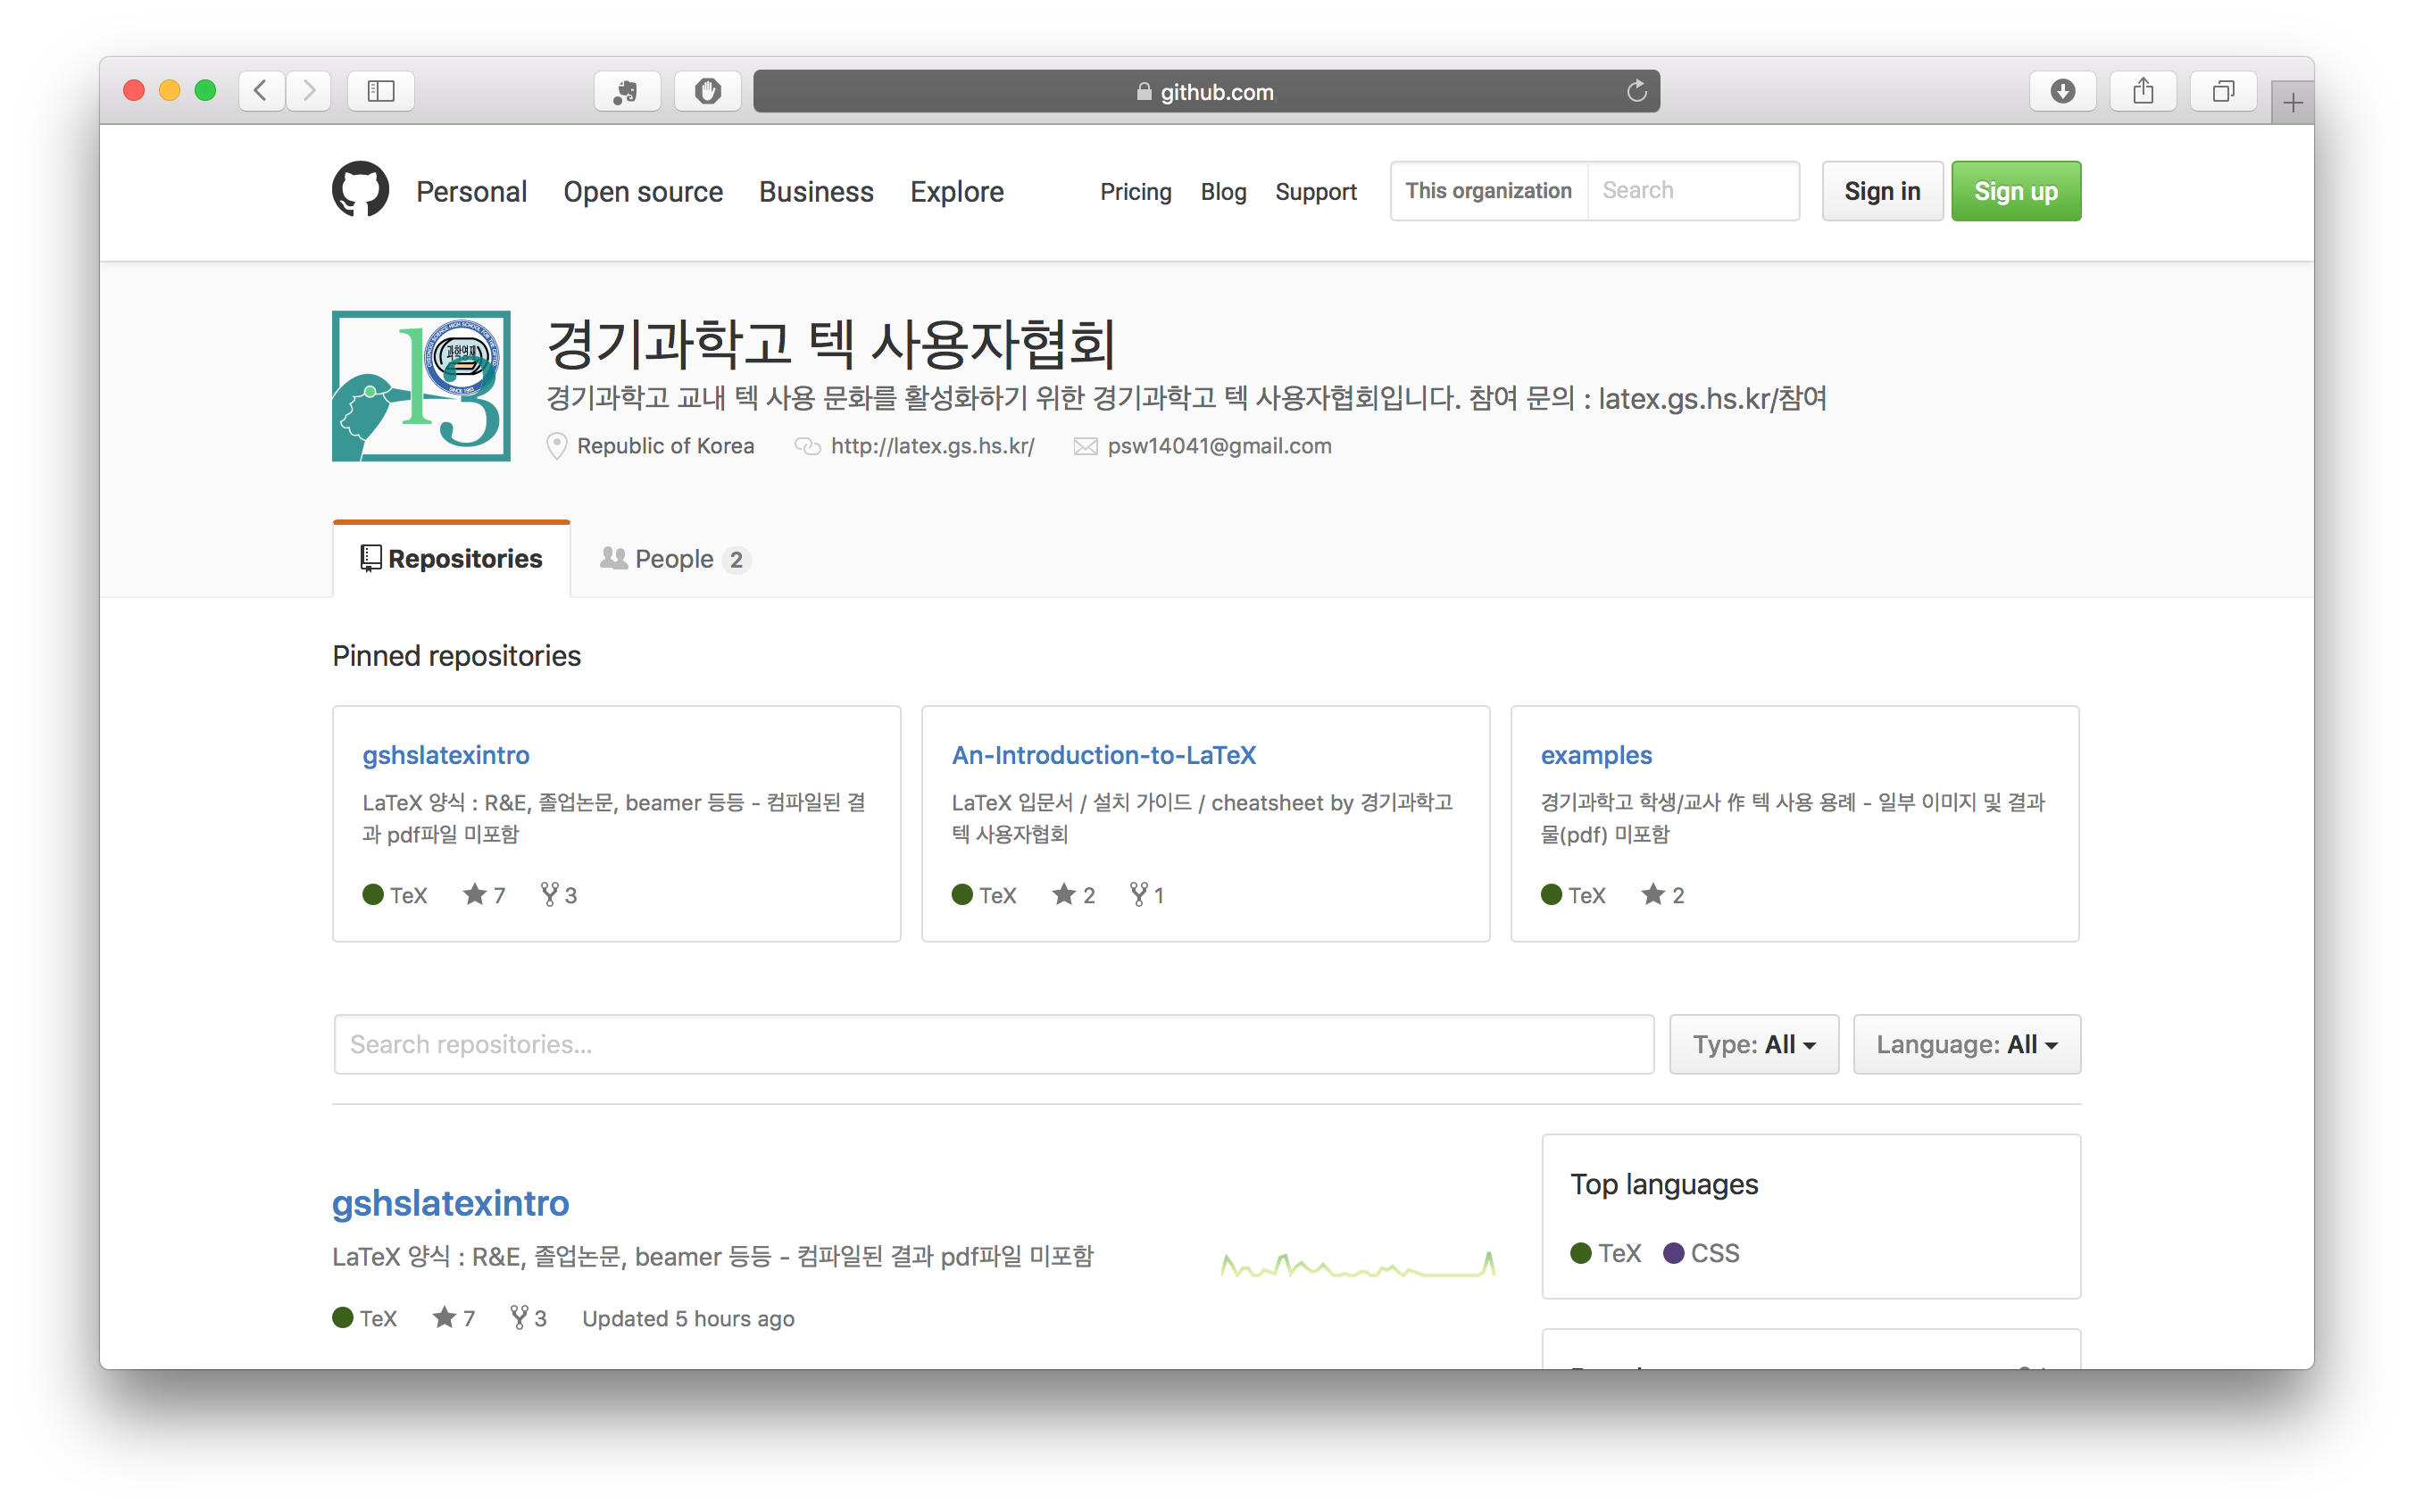
\includegraphics[width=\textwidth]{GitHub_gshslatexintro.png}
	\end{center}
\end{frame}
\begin{frame}{GitHub}
	\framesubtitle{GitHub를 통한 협업 - 예시}
	\begin{center}
		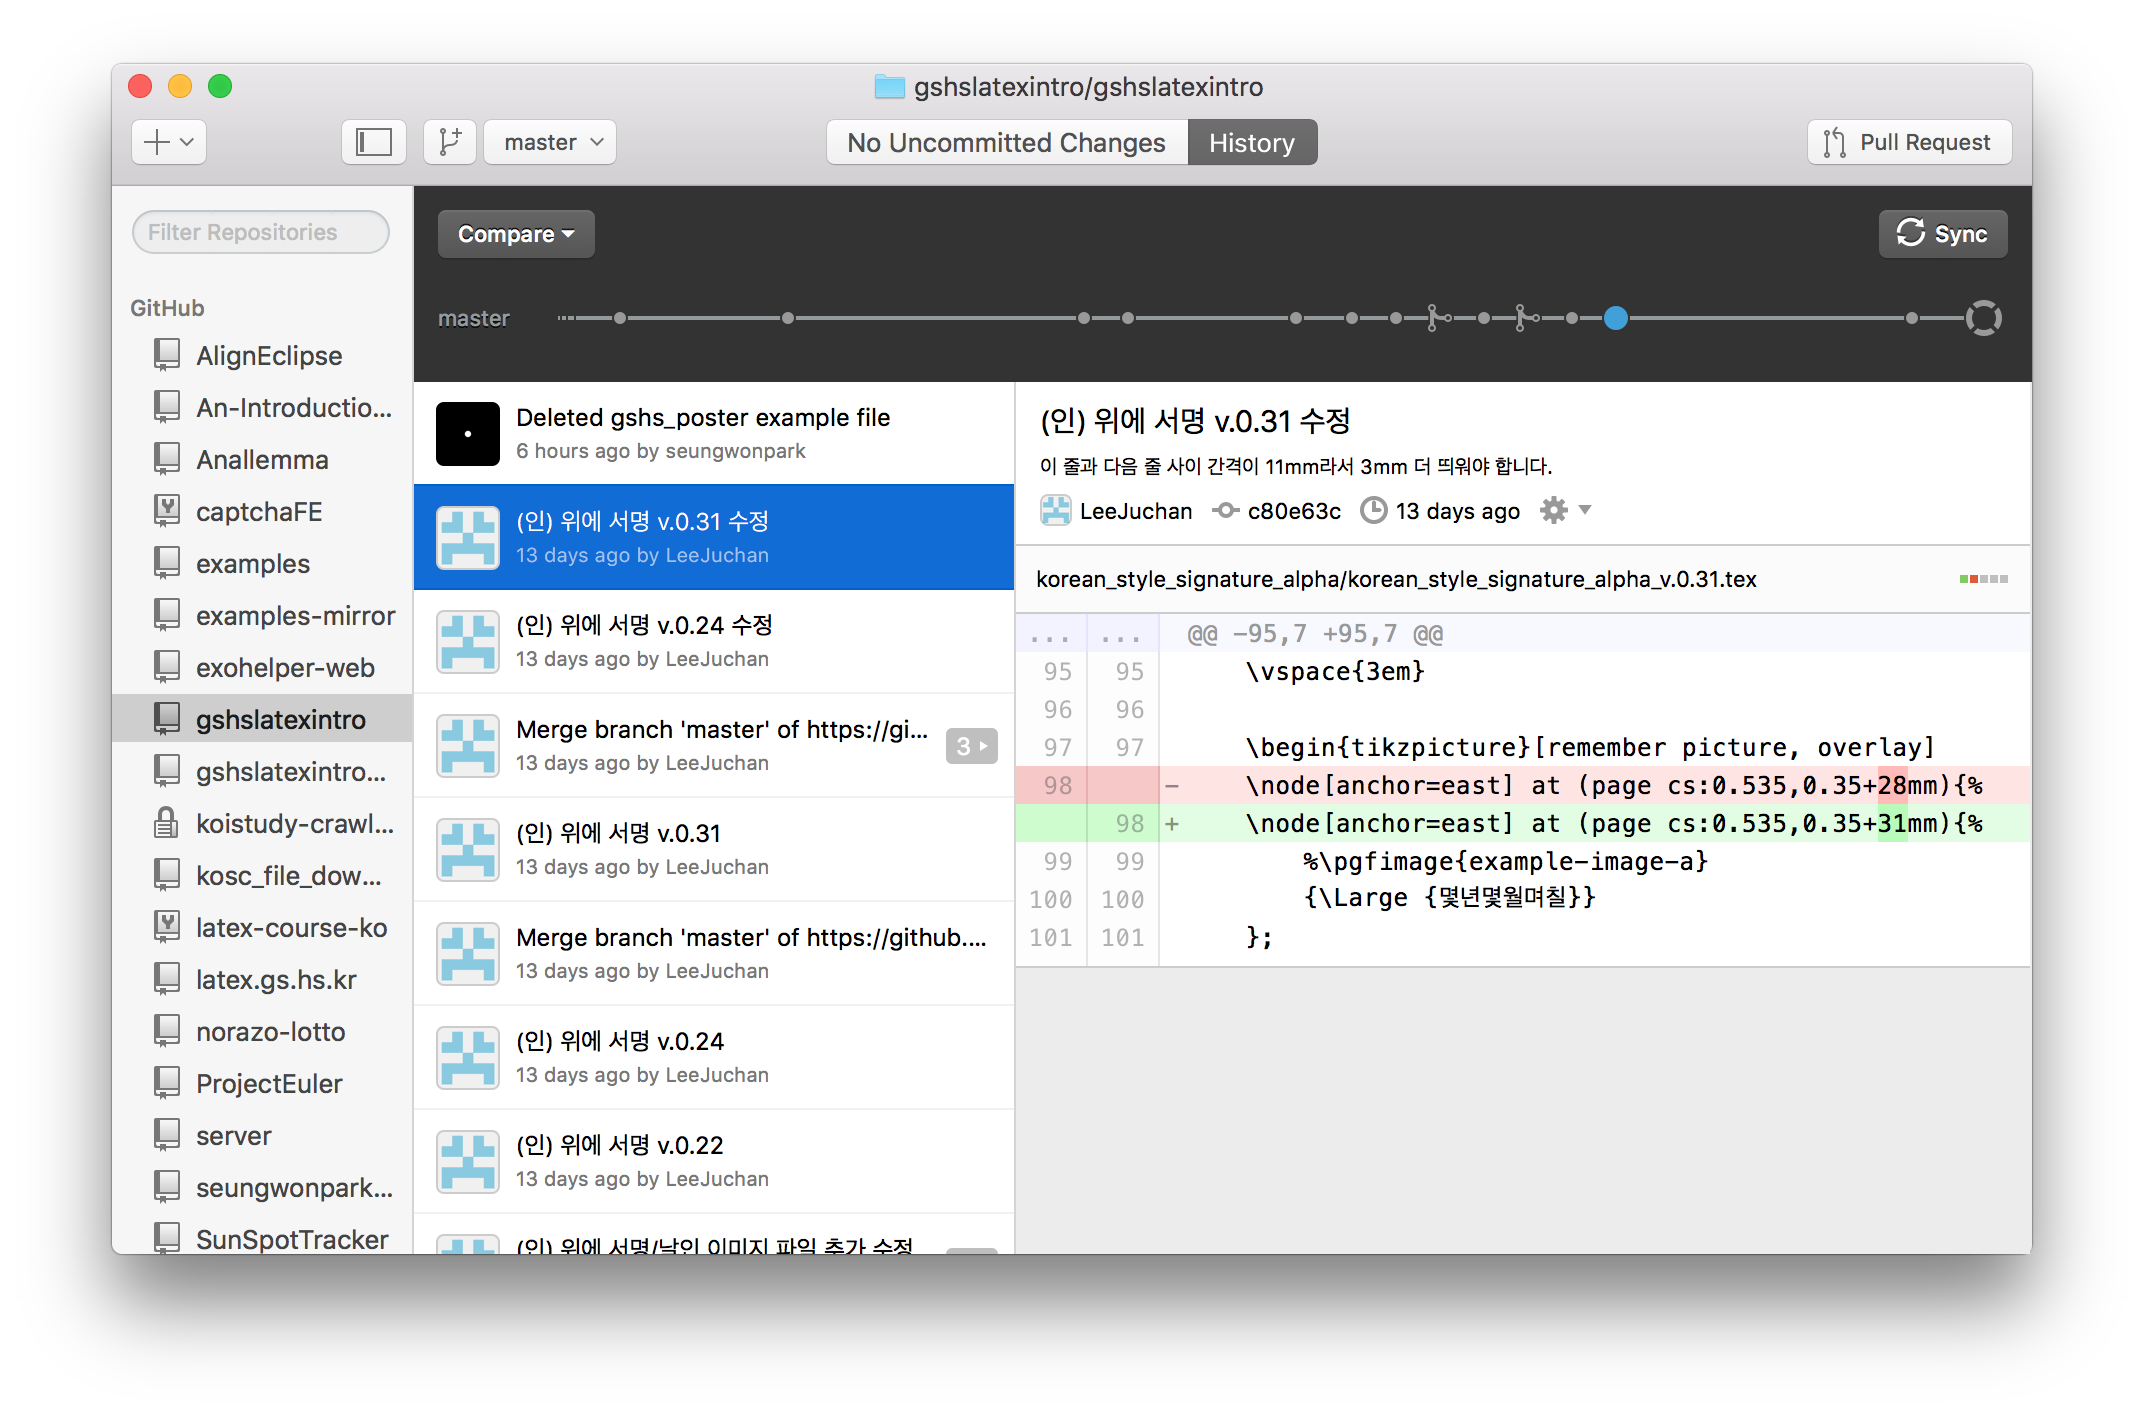
\includegraphics[width=\textwidth]{GitHub_example.png}
	\end{center}
\end{frame}
\begin{frame}{`회원'}
	\begin{center}
		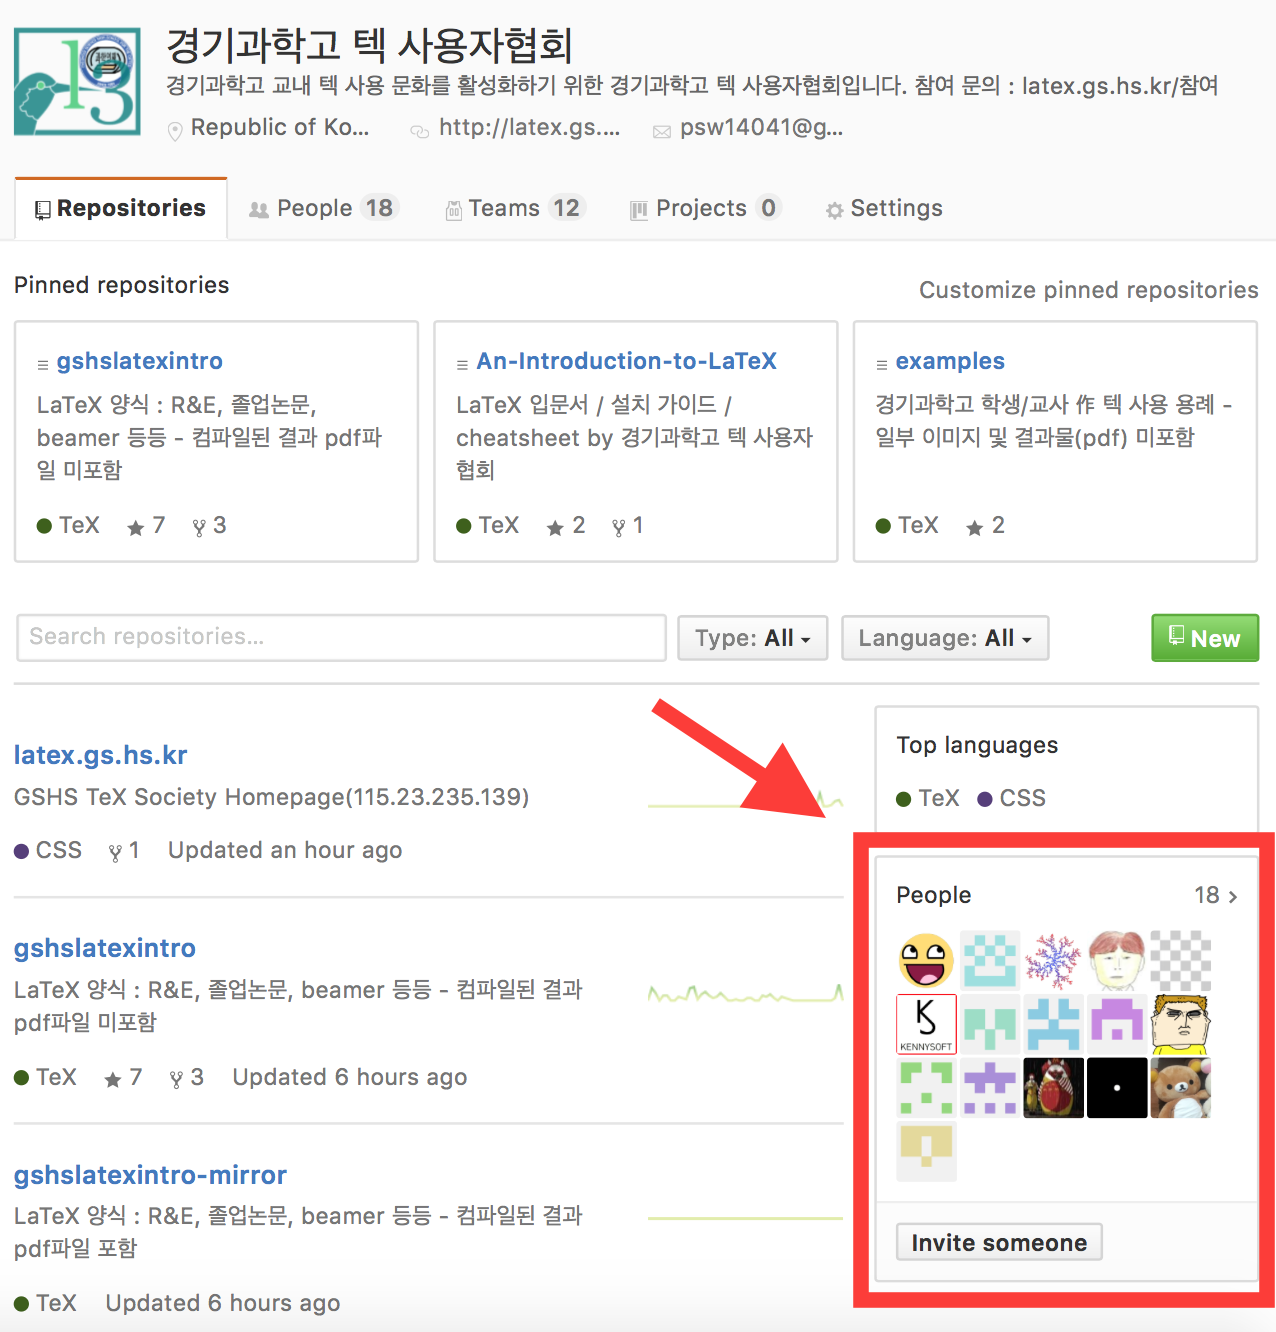
\includegraphics[width=.7\textwidth]{GitHub_gshslatexintro_people.png}
	\end{center}
\end{frame}
\begin{frame}{`회원'이 되기 위해서는}
	\begin{itemize}
		\item 협회 규범집 제 2조(`협회 회원에 관하여') 전문 : \url{https://git.io/vMbrg}
		\item 경기과학고 구성원이라면 누구든지 기존 회원의 초대를 통해,
		협회의 GitHub organization에 join하여 회원이 되고 활동에 참여할 수 있다.
	\end{itemize}
	\begin{itemize}
		\item `\url{latex.gs.hs.kr/참여}참여' 참조 바람.
	\end{itemize}
\end{frame}
\section{Repository별 특성}
\begin{frame}{개요}
	협회의 주요한 GitHub 저장소(repository)는 총 6개.
	\begin{itemize}
		\item gshs-format : 각종 양식파일
		\item gshs-format-mirror : + 컴파일된 결과물 포함
		\item examples : 각종 텍 용례
		\item examples-mirror : + 컴파일된 결과물 포함
		\item An-Introduction-to-LaTeX : \LaTeX\ 입문서
		\item latex.gs.hs.kr : 홈페이지 소스 코드
	\end{itemize}
	이 절에서는 각 repo.의 특성을 기술한다.
\end{frame}
\subsection{gshs-format}
\begin{frame}{gshs-format}
	정보
	\begin{itemize}
		\item 한글명 : `양식'
		\item 다른 모든 repo.가 비롯되어 온 오래된 repo.
		\item R\&E 보고서, 졸업논문, 휴텍 등의 \TeX 양식.
	\end{itemize}
	\vfill
	유의사항
	\begin{itemize}
		\item 저용량을 원칙으로 한다.
		\item 컴파일된 결과물, 대용량 파일은 mirror에 첨부.
		\item repo.의 이름이 organization 이름과 동일함에 유의
	\end{itemize}
	\vfill
\end{frame}
\subsection{examples}
\begin{frame}{examples}
	정보
	\begin{itemize}
		\item 한글명 : `예제'(구 : `예시 코드')
		\item 매나니 강의, 나코더 문제/해설지, 각종 레포트 등의 예제
		\item `남이 짜놓은 코드 보며 배우자'
		\item \TeX\ 으로 고퀄의 문서를 만들었다면\ldots 공유!
	\end{itemize}
	\vfill
	유의사항
	\begin{itemize}
		\item 컴파일된 결과물, 대용량 파일은 mirror에 첨부.
	\end{itemize}
	\vfill
\end{frame}
\subsection{An-Introduction-to-LaTeX}
\begin{frame}{An-Introduction-to-LaTeX}
	정보
	\begin{itemize}
		\item 한글명 : `텍 입문서'
		\item ver2.0 : beamer(발표자료) 형식의 입문서
		\begin{itemize}
			\item Day0, Day1, Day2, Day3, \ldots
			\item Installation : 텍 사용환경 준비 가이드
			\item Contribution : 지금 보고 있는 이 문서.
		\end{itemize}
		\item cheatsheet : \TeX 초심자를 위한 커닝페이퍼
	\end{itemize}
	\vfill
	유의사항
	\begin{itemize}
		\item 입문서는 간략하면서도 필요한 내용을 전달해야.
		\item lshort-kr과 차별을 두어야 함.
	\end{itemize}
	\vfill
\end{frame}
\subsection{$ \ast $-mirror}
\begin{frame}{$ \ast $-mirror}
	정보
	\begin{itemize}
		\item 한글명 : `$ \ast $-미러'
		\begin{itemize}
			\item gshs-format(양식), examples(예제)가 해당됨.
		\end{itemize}
		\item 저용량을 원칙으로 하는 repo.의 대용량 버전.
		\begin{itemize}
			\item 양식의 경우 - 양식의 컴파일된 결과물 미리보기.
			\item 예제의 경우 - 예제의 결과물을 공유하는 데에 유용.
		\end{itemize}
		\item 용량 제한 없음
	\end{itemize}
	\vfill
	유의사항
	\begin{itemize}
		\item $ \ast $에 올린 것은 반드시 $ \ast $-mirror에도 올릴 것.
	\end{itemize}
	\vfill
\end{frame}
\subsection{latex.gs.hs.kr}
\begin{frame}{latex.gs.hs.kr}
	정보
	\begin{itemize}
		\item 한글명 : (없음)
		\item 협회 홈페이지의 소스 코드. Jekyll 기반.
		\item 누구나 이 repo.를 통해 홈페이지 내용을 편집 가능.
		\item 모든 수정사항/게시글은 매 분 00초에 업데이트됨.
		\item 자세한 서버 정보는 repo.의 Wiki를 참조 바람.
	\end{itemize}
	\vfill
	유의사항
	\begin{itemize}
		\item 학교는 엄연한 공교육 기관.
		\begin{itemize}
			\item 서버, 도메인 모두 학교 소속이니, 웹페이지에 부적절한 내용이 있어서는 안됨.
			\item \TeX\ 과 무관한 것에 이 서버/도메인을 사용하는 것 또한 금지됨.
		\end{itemize}
	\end{itemize}
	\vfill
\end{frame}
\subsection{기타(Misc.)}
\begin{frame}{기타(Misc.)}
	latex-course-ko
	\begin{itemize}
		\item Korean translation of ``An interactive introduction to LaTeX using Overleaf.''
		\begin{itemize}
			\item Original : \url{http://bit.ly/1JNiWqf}
		\end{itemize}
	\end{itemize}
	\vfill
	gshslatexintro.github.io
	\begin{itemize}
		\item 구 홈페이지 소스 코드 및 도메인.
		\item 사용 종료 중이지만 리다이렉트를 위해 삭제 금지.
		\item 아래는 모두 \url{latex.gs.hs.kr}로 리다이렉트됨.
		\begin{itemize}
			\item \sout{\url{gshslatexintro.github.io/gshslatexintro}}\footnote{2017.03.14 20:00 경 gshslatexintro repo.가 gshs-format으로 변경되며 삭제됨}
			\item \url{gshslatexintro.github.io}
			\item \url{chanspi.ddns.net/gshs/LaTeX}
		\end{itemize}
	\end{itemize}
	\vfill
\end{frame}
\end{document}